\section{Dataset - European Cloud Cover }
%This chapter presents the developed methodology used in the compilation of the dataset. 
This section presents the developed algorithms necessary for the compilation of the dataset \acrfull{ecc}. It is pieced together from two sources, reanalysis, \acrshort{era5} and \acrfull{msg} cloud mask. The common period of 2004 to 2018 is selected and downloaded size is 17Gb, stored in \acrshort{netcdf}-files.


Several candidate satellites were considered before arriving at the combination of datasets presented in this chapter. Spatiotemporal consistency and resolution were given top priority. 
Reanalysis is as close one can get to observations continuous in time and space. All reanalysis product are different. They all depend on the forecast assimilation system used and observations assimilated. There are multiple global datasets available (\cite{Fujiwara2017IntroductionSystems}). \acrshort{era5} was elected 
%over, JRA \textbf{må siteres} and MERRA \textbf{må siteres}, 
because of it's fine resolution and resent release date of January 2020. The assimilation model used, the \acrshort{ifs}-model is a state-of-the-art \acrshort{nwp}-model. As of now, few experiments have been conducted on this data. It is therefore more exciting to explore this datasets ability to perform climate predictions using data driven learning.
%above JRA and MERRA because of the spatial resolution and because it the latest within reanalis products available. 

The variable cloud mask is provided by many satellites, bringing valuable information in itself, but also for the retrieval of other variables restricted to cloud free conditions, such as humidity. The satellite product chosen for this project is the \acrfull{msg}. This satellite is in geostationary orbit, and has an exceptional temporal resolution, with scans every 15min. Knowing that the average lifetime of a cloud is 60min or less, the selected data set was found to be the most suitable for the purpose of this study (\cite{lohmann2016}, p. 19). The finished dataset, described in detail below, is named \acrfull{ecc}. 

\subsection{Domain}
The geographical domain has, for this project, been restricted to latitude, $\theta \in[30,50]$ and longitude $\phi \in [-15, 25]$. The resulting dimensions of the grid become $81\times161$ pixels. Figure \ref{fig:map} shows the domain included in this dataset. The domain covers Central Europe and North Africa. $54\%$ of the domain is land, and $46\%$ is ocean or sea. 
\begin{figure}[h]
    \centering
    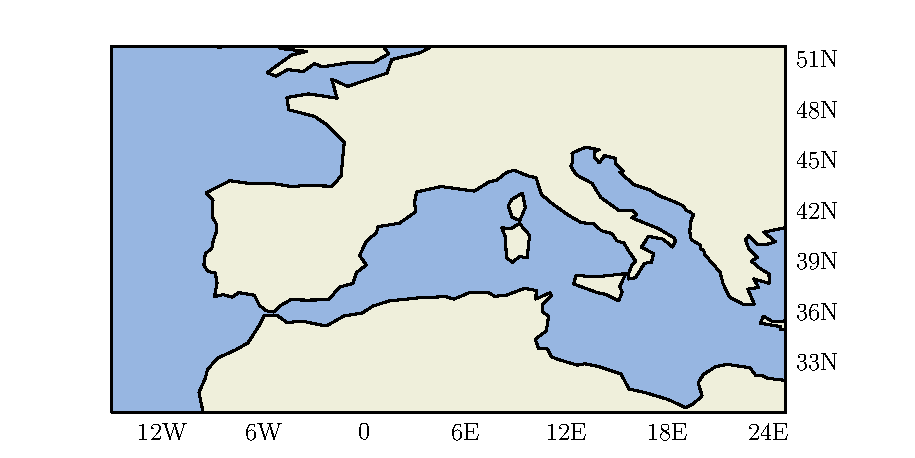
\includegraphics[scale = 1.0]{python_figs/Domain.pdf}
    \caption{Map showing the domain in the projection available in \acrshort{ecc}.}
    \label{fig:map}
\end{figure}

\subsection{Physical basis of variable decision} \label{sec:ecc}
The overall goal is to investigate whether basic meteorological variables such as temperature, pressure and humidity are sufficient for prediction of cloud fractional cover with a reasonable accuracy. Cloud dynamics is far more complicated than what can be describes by these variables, as discussed in Section \ref{sec:cloud_in_climate_system}.
%The condition describing what is ``sufficiently accurate'' is further explained in Chapter \ref{ch:computer_experiments}.

This project is a \textit{proof of concept study} aimed to demonstrate the feasibility of using \acrshort{ai} to parameterize \acrshort{cfc}. Employing data driven learning to represent cloud physics and dynamics in its full complexity requires measurements from technologies not yet invented. If they did exist, the computational cost would be large and there is no guarantees of state-of-the-art performance. However, large amounts of data is collected on a daily basis. Understanding how to utilize the information in these measurements despite its flaws (gaps and artifacts) is of major importance. 

Precipitation formation and cloud optical thickness are affected by changes on a microphysical level. However, they are undeniably closely related to the macrophysical properties of the cloud as well. Imagine precipitation without a cloud fractional cover. 

Reliable estimates of large-scale variables are available from using reanalyses or other climate models. Restricting the focus here to the macrophysical aspects of clouds makes it reasonable to choose these as explanatory variables, thereby ensuring that it is possible to build usable application of this parameterization in the future.

For this dataset, all these large-scale variables are produced by \acrshort{era5}. Some variables have been chosen because they are reliable and fundamental meteorological variables, e.g. temperature and surface pressure. Others were chosen because they are essential in cloud formation, e.g. specific and relative humidity. The variables were all retrieved from the surface or the closest pressure level (1000hPa). The rest of this section gives a brief introduction to their role in cloud formation.

From the weather maps on the news, low and high pressure systems might be familiar terms. Low pressure systems are often associated with precipitation, while high pressure systems are associated with nice weather. The Earth is not equally heated due to the its spherical geometry. Warmer air rises, generating a low pressure at the surface. As the air rises the temperature within the rising air parcel decreases. From Equation \eqref{eq:clausius_clapeyron} it can be shown that colder air can retain less vapor, enhancing the rate at which saturation is achieved. Under supersaturated conditions some of the vapor condenses, generating cloud water, forming a cloud, and occasionally precipitation. Low latitudes and the mid-latitudes of the summer hemisphere are often associated with this type of convective motions, generating cumulus type clouds. 
%\textbf{TS: Viktig å også si noe kort om storskala sirkulasjon, siden diskusjonen ovenfor fokuserer på lokale prosesser. Over Sahara (som jo kommer inn i domenet ditt) er det for eksempel varmt, men lite skyer og nedbør fordi dette er et område med storkskala nedsynkning}

In areas of lower pressure, the surrounding air will flow toward the low pressure center to offset the pressure difference. Induced by Earth's rotation the Coriolis effect forces winds of low pressure systems to swirl counterclockwise north of the equator and clockwise south of the equator, causing an accumulation of air in the center of low pressure system, pushing it to higher altitudes in the atmosphere. A high pressure system exhibits the exact opposite behavior, it swirls in the reverse direction, and the air flows from the center. Diverging air masses cause sinking motions of parcels from higher in the atmosphere to fill the void. 

The large scale circulation generate zonal bands of sinking and rising air masses. Warm air rises at the equator as a result of the Earths' spherical geometry, this air move poleward, cools and sinks. The Saharan desert is located in an area of sinking air masses. Despite its warm temperatures, there is little to no cloud formation and associated precipitation in this region. 

\textbf{In zones of rising air, bands of low pressure systems are concentrated on fronts.} A front is a transition zone between two types of air masses, usually of different temperatures. % A cold front is formed when warmer air is pushed to higher altitudes, this is known to generate clouds, which is often assosiated with precipitation. % TS: Her følte jeg at det manglet noe om fronter som jo er hvor skyene er konsentrert i forbindelse med lavtrykk.
Large cloud decks are generated from the lifting of entire layers. This is likely to happen when the air is forced to higher altitudes by fonts (warm and cold) or orography (\cite{lohmann2016}, p. 79). Norway lies within the prevailing westerlies a band or rising air. Low pressure systems frequently appear along the coast from the Atlantic sea, resulting in a cloudy and wet region. 
% The warm moist air associated with the gulf stream amplifies this effect. Winds transports the substances suspended in air, such as pollutants and humidity. 

The dataset includes both relative and specific humidity. Relative humidity is a measure of how much vapor the air contains, relative to how much it can hold at a certain temperature. At relative humidity of 1 the air is at its dew point, and for higher values clouds form. These conditions are commonly referred to as supersaturated, consequently the variable relative humidity is ``limited'' to the range from 0 to 1. 
%under such supersaturated conditions it is often referred to as \textbf{X}, and 
%Therefore it is common to limit the range of relative humidity to be between 0 and 1. 
However the variable is still a measure of the identical ratio, and this explains why values exceeding 1 is present in the dataset. Relative humidity is unitless and for higher values the air is more humid.

Specific humidity is the ratio between mass of vapor and mass of air, with unit of $kg kg^{-1}$ (\cite{lohmann2016}, pp. 53-54). Whether relative or specific humidity is the better predictor is not clear a priori. The data is gathered from the model level closest to the surface, at an altitude of 1000hPa. For large scale motions, when friction and the centrifugal force are less important, the wind field can be derived from the pressure gradients, this is know as geostrophical winds  (\cite{lohmann2016}, pp. 81-84).

Observed weather systems depend upon local and large scale interaction between variables. Different combinations are thought to explain different cloud conditions. For instance surface pressure is thought be a good predictor of frontal systems. The surface humidity, however, is not thought to play a big role in saturating the airmasses, since they appear so high in the atmosphere. Consequently, humidity is expected to have a low predictability for such an event. 
%Cold front occurs where cold air replace warm air, and warm front is the opposite process. 

In shallow (and deep) convection systems, the air rises from the surface and the temperature and surface humidity is though to explain this phenomena well. Rising airmasses will in turn generate low pressure at the surface. The variables temperature, humidity and pressure are assumed to be reasonable predictors for convective activity and the cumulus clouds responsible for afternoon showers.
%\textbf{The large scale surface variable pressure can provide useful information for detecting fronts, and wind patterns potentially revealing usfull information in prediction the movement of clouds. Temperature is thought to revels cumulus type clouds in regions without sinking air masses. }. \textbf{Due to the combination of large and small scale patterens its important to study the geographical distribbution of the best model.}
%\textbf{Can make heatmap showing the best model, one color at a time. }
%TS: Her trengs en tydeligere diskusjon av hvilke skytyper man forventer at de storskala bakke-varaiblene er mest relevante for, og hvilke de eventuelt er mindre
%\textbf{Check out clouds in the IPCC hvor de beskriver hva som er problemet med de ulike %parameteriseringene.}

\subsection{Area Weighting Regridding Scheme (AWRS)} \label{sec:remapping}
Computing cloud fractions based on the cloud mask requires a regridding scheme. Common schemes for solving similar tasks are mean, nearest neighbor or area weighting. For this particular task, the pixels are of uneven size and the area weighted scheme seemed most appropriate. 

This section provides a step-by-step description of the necessary data processing done for the compilation of \acrshort{ecc}, transforming clouds masks provided in \textit{space-view} to cloud fractions on a uniform grid. \acrshort{eumetsat} doesn't provide suitable software to tackle this particular task (personal communication EUMETSAT staff). Building the dataset requires the implementations of software with functionality to perform the regridding, described in detail below, named the \acrfull{awrs}.

The regridding algorithm consists of two modules; \textit{(1) detection} and \textit{(2) area weighting algorithm}. Let the subscripts denote the dataset pertaining to a particular grid. Grid\textsubscript{MSG} refers to the space-view grid of the \acrlong{msg} and grid\textsubscript{ECC} refers to the uniform grid originating from \acrshort{era5}. Note that grid\textsubscript{ECC} is identical to  grid\textsubscript{\acrshort{era5}}. The \textit{detection algorithm}, computes the co-location of pixels across grid and determines the contributing pixel from grid\textsubscript{MSG} to grid\textsubscript{\acrshort{era5}}.

The pixels are then classified into the different categories such as \textit{corner}, \textit{center}, \textit{left}, \textit{right}, \textit{upper} and \textit{lower boundary}. These categories are later used to isolate the portion of the pixel contributing to grid\textsubscript{ECC}.
The second module, \textit{the area weighting}, consist of the category based area weighting algorithm based on the developed equations.

\subsubsection{Equations describing grid area}
Since Earth is spherical the pixels areas are computed using spherical coordinates. Figure \ref{fig:spherical_coords} shows a square projected on to a sphere. Deriving the equation for computing the area of a square in spherical coordinates, requires integrating over changes in latitude, $d\theta$ and longitude, $d\phi$. In Equation \eqref{eq:sphere_integral} the variables of integration are given a prime to keep them distinct from the integration boundaries.
\begin{figure}
    \centering
    
    
\tdplotsetmaincoords{60}{110}
%
\pgfmathsetmacro{\rvec}{1.0}
\pgfmathsetmacro{\thetavec}{30}
\pgfmathsetmacro{\phivec}{60}

\pgfmathsetmacro{\deltathetavec}{40}
\pgfmathsetmacro{\deltaphivec}{80}

%
\begin{tikzpicture}[scale=5,tdplot_main_coords]
    \coordinate (O) at (0,0,0); % origo
    \coordinate (z) at (0, 0, 1.0); % origo
    %\draw[thin, <->] (1, 0.7, 1.16) -- (1, 0.52, 1.2) node[pos = 0.8, above right]{\Large $d\theta$};
    
    \draw[very thick,->] (0,0,0) -- (1.7, 0, 0) node[anchor=north east]{\Large $x$};
    \draw[very thick,->] (0,0,0) -- (0, 1.7, 0) node[anchor=north west]{\Large $y$};
    \draw[very thick,->] (0,0,0) -- (0, 0, 1.7) node[anchor=south]{\Large $z$};
    
    \shade[ball color = teal, opacity = 0.1] (0,0,0) circle [radius=\rvec];
    \draw (0,0,0) circle [radius=\rvec];
    
    \tdplotsetcoord{P}{\rvec}{\thetavec}{\phivec}
    \tdplotsetcoord{dP}{\rvec}{\deltathetavec}{\phivec}
    
    \tdplotsetcoord{G}{\rvec}{\thetavec}{\deltaphivec}
    \tdplotsetcoord{dG}{\rvec}{\deltathetavec}{\deltaphivec}

    \draw[very thick, color=teal, opacity = 0.3] (O) -- (G) node[above right]  {};
    \draw[very thick, color=teal, opacity = 0.6] (O) -- (dG) node[above right] {};    
    \draw[very thick, color=red, opacity = 0.6] (O) -- (P) node[above left]  {\Large $R$};
    \draw[very thick, color=teal, opacity = 0.6] (O) -- (dP) node[above right] {};
    
    \draw[dashed, color=teal] (O) -- (Pxy);
    \draw[dashed, color=teal] (dP) -- (Pxy);
    %\draw[dashed, color=red] (Pz) -- (Py);

    %\draw[dashed, color=red] (dP) -- (Pxy);
    
    \draw[very thick, color=red] (O) -- (Gxy) node[above right] {\Large $Rcos\theta$};
    \draw[dashed, color=teal] (dG) -- (Gxy);
    %\draw[dashed, color=black,looseness = 10, bend left] (z) -- (G)  node[pos = 0.6, above right] {\Large $Rsin\theta$};
    \draw[dashed, color=teal,looseness = 10, bend left] (z) -- (G);
    \draw[dashed, color=teal, bend right] (P) -- (z);
    
    
    \draw [very thick, color=blue] (\phivec:0.5)  arc (\phivec:\deltaphivec:0.5) node [below right, pos=0.3] {\Large $Rcos\theta d\phi$};

    
    %\tdplotdrawarc[tdplot_rotated_coords, ->]{(dP)}{.7}{(Pxy)}
    
    \draw[dashed, very thick, color=teal, fill = teal, opacity = 0.2] (P) -- (dP) -- (dG) -- (G) -- (P);
    \draw[dashed, very thick, color=teal] (P) -- (dP) -- (dG) -- (G) -- (P);
    \draw[very thick, color=blue] (dG) -- (G) node[pos = 0.5, above right] {\Large $Rd\theta$};
    \draw[dashed, color=teal] (dG) -- (G);    \tdplotdrawarc[]{(O)}{0.4}{0}{\phivec}{anchor=north}{\Large $\phi$}
    %\tdplotdrawarc{(O)}{0.2}{0}{\deltathetavec}{anchor=north}{$\theta$}

    \tdplotsetthetaplanecoords{\phivec};
    
    %\tdplotdrawarc[tdplot_rotated_coords]{(0,0,0)}{0.8}{0}%
        %{\thetavec}{anchor=south west}{\Large $\theta$};
    
    \tdplotdrawarc[tdplot_rotated_coords, pos = 0.01]{(0, 0.5, -0.3)}{0.45}{0.0}%
        {\thetavec}{anchor=south west}{\Large $\theta$};
    
    \tdplotdrawarc[tdplot_rotated_coords, pos = 0.5]{(0,0,0.2)}{0.26}{0}%
        {\thetavec}{anchor = south west,shift={(4mm,-5mm)}}{\Large $d\theta$};
        
    %\tdplotdrawarc[tdplot_rotated_coords, <->]{(0.1, 0.2, 0)}{.5}{0}{\thetavec}{anchor=east}{\Large $d\theta$}
    \shade[ball color=teal,tdplot_screen_coords,opacity=0.2] (O) circle[radius=\rvec];
    \foreach \X/\Y in {xy/z,yz/x,zx/y}
        {\begin{scope}[canvas is \X\space plane at \Y=\rvec]
         \fill circle[radius=1pt];
        \end{scope}}
    \end{tikzpicture}
    \caption{Mathematical properties of a square projected onto a sphere.}
    \label{fig:spherical_coords}
\end{figure}
The general expression for the area of a square in spherical coordinates, is given by the following integral,
\begin{equation} \label{eq:sphere_integral}
    A = R^2\int_{ \theta - \delta \theta }^{\theta + \delta \theta} \int_{ \phi - \delta \phi }^{\phi + \delta \phi} cos\left( \theta' \right) d\phi' d\theta'
\end{equation}
%This can be rewriting into, \textbf{needs indices $(i, j)$ ..?}
the equation can be rewritten into,
\begin{equation} \label{eq:sphere_finish}
    A \left( \theta, \phi, \delta \theta, \delta \phi   \right)= 2R^2 \left( sin\left( \theta + \delta \theta  \right) - sin\left(  \theta - \delta \theta  \right) \right) \delta \phi
\end{equation}
where $R=6378km$ denotes the distance to Earth's center, $\theta$ the latitude and $\phi$ the longitude. Equations \eqref{eq:sphere_integral} and \eqref{eq:sphere_finish} can be related to Figure \ref{fig:spherical_coords} by setting $d \theta = 2 \delta \theta$ and $d \phi = 2 \delta \phi$. The implementation is scaled by $R$.

The equations used to compute the area weighted cloud fractional cover are as follows,
\begin{equation} \label{eq:area_weighting}
    CFC_{ECC} = \frac{1}{A} \sum_{i=0}^{N} a_i m_i
\end{equation}
where,
\begin{equation} \label{eq:tot_area}
    A = \sum_{i=0}^{N} a_i
\end{equation}
Inserting $m_i = 1$ $\forall$ $i \in [0,N]$ into Equation \eqref{eq:area_weighting} results in $CFC_{ECC}=1$, independent of $a_i$, proving that the minor overlap between pixels in Figure \ref{fig:pixels_contributing_to_cell} does not affect the range of cloud fractions, which remains between 0 and 1.

\subsubsection{Estimating properties of grid\textsubscript{MSG}}
% Estimating the extent of the cell.
The coordinate information is provided in grids of latitudes, $\theta$ (degrees north), and longitudes, $\phi$ (degrees east) values. The coordinate represents the center of a pixel. To acquire the information about the extent of cells in a non-uniform grid requires some simplifications. 

%%%%%%%%%%%%% PART ONE
Computing the area weighted average of cloud masks requires detecting the pixels of grid\textsubscript{MSG}
contributing to the grid\textsubscript{\acrshort{era5}} cell, and computing their area. The pixels are classified into five categories; \textit{center}, \textit{left}, \textit{right}, \textit{up} and \textit{down boundary}.
%The detection algorithm is straight forward, overlapping pixels are included and labelled with a suitable category.
The cloud mask pixels are smallest at the nadir point, increasing in all directions. Figure \ref{fig:estimate_dlon} illustrates this by showing an example of three neighboring pixels. In this example the apparent pixel size increases going eastward. Consequently, there is an asymmetry between neighboring pixels. The distance from the center to the right and left neighbor is unequal. In order to take advantage of the analytical expression derived in Equation \eqref{eq:sphere_finish}, the extent of a contributing pixel is approximated by averaging the right and left distances. The categorization is illustrated in Figure \ref{fig:pixels_contributing_to_cell} using different colors.

\tdplotsetmaincoords{60}{110}
%
\pgfmathsetmacro{\rvec}{1.6}
\pgfmathsetmacro{\thetavec}{30}
\pgfmathsetmacro{\phivec}{60}

\pgfmathsetmacro{\deltathetavec}{40}
\pgfmathsetmacro{\deltaphivec}{80}

\begin{figure}
    \centering
    
    
\tdplotsetmaincoords{60}{110}
%
\pgfmathsetmacro{\rvec}{1.0}

\pgfmathsetmacro{\thetavec}{30}
\pgfmathsetmacro{\deltathetavec}{40}
\pgfmathsetmacro{\deltatwothetavec}{50}
\pgfmathsetmacro{\deltathreethetavec}{60}

\pgfmathsetmacro{\phivec}{-30}
\pgfmathsetmacro{\deltaphivec}{10}
\pgfmathsetmacro{\deltatwophivec}{50}
\pgfmathsetmacro{\deltathreephivec}{90}



\begin{tikzpicture}[scale=5,tdplot_main_coords, 
                    mycirc/.style={circle,fill=blue!20, minimum size=0.5cm}]

    %%%%%%%%%%%%%% Setting up axis and coordinate system.
    \coordinate (O) at (0,0,0); % origo
    \coordinate (z) at (0, 0, \rvec); % origo
    %\draw[thin, <->] (1, 0.7, 1.16) -- (1, 0.52, 1.2) node[pos = 0.8, above right]{\Large $d\theta$};
    \draw[very thick,->, opacity = 1.] (0,0,0) -- (1.7, 0, 0) node[anchor=north east]{\Large $x$};
    \draw[very thick,->,  opacity = 1.] (0,0,0) -- (0, 1.7, 0) node[anchor=north west]{\Large $y$};
    \draw[very thick,->,  opacity = 1.] (0,0,0) -- (0, 0, 1.7) node[anchor=south]{\Large $z$};
    \shade[ball color = teal, opacity = 0.1] (0,0,0) circle [radius=\rvec];
    \draw (0,0,0) circle [radius=\rvec];

    
    \tdplotsetcoord{a}{\rvec}{\deltathetavec}{\phivec}
    \tdplotsetcoord{b}{\rvec}{\deltatwothetavec}{\phivec}
    % Changeing the rightmost part 
    \tdplotsetcoord{c}{\rvec}{\deltathetavec-5}{\deltaphivec}
    \tdplotsetcoord{d}{\rvec}{\deltatwothetavec+5}{\deltaphivec}
    
    \draw[dashed, very thick, color=teal, fill = teal, opacity = 0.2] (a) -- (b) -- (d)-- (c) -- (a);
    \draw[dashed, very thick, color=teal] (a) -- (b) -- (d)-- (c) -- (a);

    \tdplotsetcoord{a}{\rvec}{\deltathetavec-5}{\deltaphivec}
    \tdplotsetcoord{b}{\rvec}{\deltatwothetavec+5}{\deltaphivec}
    \tdplotsetcoord{c}{\rvec}{\deltathetavec-10}{\deltatwophivec}
    \tdplotsetcoord{d}{\rvec}{\deltatwothetavec+10}{\deltatwophivec}
    
    \draw[dashed, very thick, color=teal, fill = teal, opacity = 0.2] (a) -- (b) -- (d)-- (c) -- (a);
    \draw[dashed, very thick, color=teal] (a) -- (b) -- (d)-- (c) -- (a);
        
    % First column
    %\node[draw] at (0, -2)  (c)     {C};
    %\node[draw] at (0.3, -0.25, 0.5) {$\phi_{(i,j-1)}$};
    %\node[draw, thick] at (0.5, 0.3, 0.65) {$\phi_{(i,j)})$};
    %\node[draw, thick] at (0.5, 0.73, 0.87) {$(i,j+1)$};
    \filldraw [teal, label=above:{$\phi_{(i,j-1)}$}]  (0.3, -0.25, 0.5) circle (1pt);
    \filldraw [teal, label=above:{$\phi_{(i,j-1)}$}]  (0.5, 0.3, 0.65)  circle (1pt);
    \filldraw [teal, label=above:{$\phi_{(i,j-1)}$}]  (0.5, 0.73, 0.87) circle (1pt);
    
    \tdplotsetcoord{a}{\rvec}{\deltathetavec-10}{\deltatwophivec}
    \tdplotsetcoord{b}{\rvec}{\deltatwothetavec+10}{\deltatwophivec}
    \tdplotsetcoord{c}{\rvec}{\deltathetavec-15}{\deltathreephivec}
    \tdplotsetcoord{d}{\rvec}{\deltatwothetavec+15}{\deltathreephivec}
    
    \draw[dashed, very thick, color=teal, fill = teal, opacity = 0.2] (a) -- (b) -- (d)-- (c) -- (a);
    \draw[dashed, very thick, color=teal] (a) -- (b) -- (d)-- (c) -- (a);
    
    \draw [decorate,decoration={brace, amplitude=12pt, mirror}, xshift=0pt, yshift=0pt]
    (0.3, -0.25, 0.1) -- (0.5, 0.83, 0.47) node [black,midway,xshift=0.2cm, yshift = -1.5cm, very thick] {\Large $\left| \phi_{i+1,j} - \phi_{i-1, j} \right| $};
    
    \draw [decorate,decoration={brace, amplitude=12pt}, xshift=0pt, yshift=0pt]
    (0.5, 0.3, 0.65) -- ((0.5, 0.5, 0.73) node [black,midway,xshift=0cm, yshift = 2.cm, very thick] {\Large $\delta \phi_{(i, j)}$};

    \tdplotsetthetaplanecoords{\phivec};
    \shade[ball color=teal,tdplot_screen_coords,opacity=0.2] (O) circle[radius=\rvec];
    \foreach \X/\Y in {xy/z,yz/x,zx/y}
        {\begin{scope}[canvas is \X\space plane at \Y=\rvec]
         \fill circle[radius=1pt];
        \end{scope}}
    \end{tikzpicture}
    
    \caption{Illustrating the relative size of three neighbouring pixels on a sphere in the \textit{space-view} grid provided by EUMETSAT. The following example explain the changes in longitude, $\phi$, varying in eastward direction, denoted $i$. The expression is shown in Equation \eqref{eq:app_lon}. 
    The same principles applies in the latitudinal direction, see Equation \eqref{eq:app_lat}.  }
    \label{fig:estimate_dlon}
\end{figure}

\begin{figure}
    \centering
    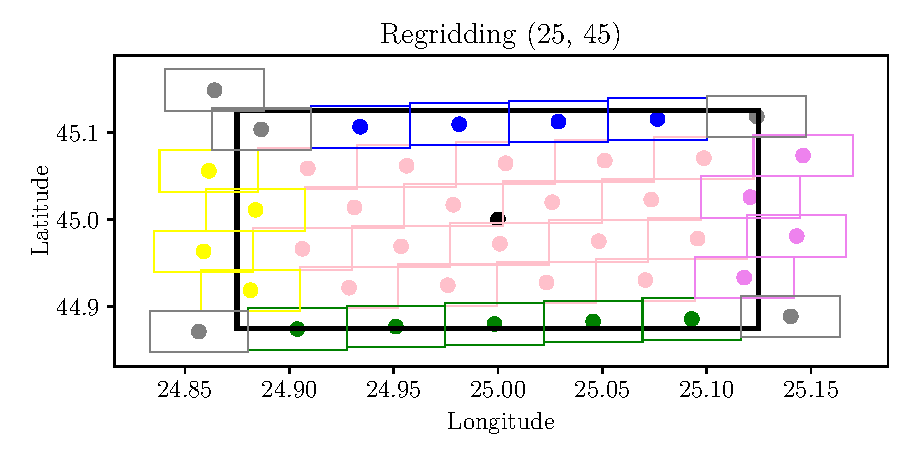
\includegraphics{python_figs/example_remapping_lat45_lon25.pdf}
    \caption{Example showing the contributing pixels to the remapping of pixel $(25, 45)$. The pixels from the satellite are classified into corner (grey), center (pink), right (purple), left (yellow), lower (green) and upper (blue) boundary. The dense black line is the pixel in grid\textsubscript{ECC}, and the other pixels shows the contributing pixels from grid\textsubscript{MSG}.}
    \label{fig:pixels_contributing_to_cell}
\end{figure}

Approximations of $d\phi$ and $d\theta$ have been made based on the two-dimensional fields of latitude and longitude values according to the below equations.
Longitudinal values vary along the first dimension, denoted with index i. The estimated half of the extent of a pixel in grid\textsubscript{MSG} is approximated by Equation \eqref{eq:app_lon}. Latitudinal changes are in north-south direction, along the second-axis, here denoted with index j. Equation \eqref{eq:app_lat} describes the distance from the center to the upper and lower boundary.
% \eqref{eq:app_lon} and  \eqref{eq:app_lat}. 
%The horizontal extent of a pixel $(i,j)$ be determined by the the averaged distance between the longitude of neighboring pixels. 
%, see Equation \eqref{eq:app_lon}. The same principles applies in the latitudinal direction, this version is shown in Equation \ref{eq:app_lat}.
\begin{equation} \label{eq:app_lon}
    \delta \phi_{i,j} = \left| \frac{\phi_{i+1,j} - \phi_{i-1, j}}{4} \right|
\end{equation}
\begin{equation} \label{eq:app_lat}
    \delta \theta_{i,j} = \left| \frac{\theta_{i,j+1} - \theta_{i, j-1}}{4} \right|
\end{equation}

The ``square'' in grid\textsubscript{MSG} resembles a trapezium, as illustrated in Figure \ref{fig:estimate_dlon}. As far as the author knows, an analytical solution for the area of a trapezium in spherical coordinates does not exist. Also, it is not clear if approximating the area with another numerical method would reduce the overall uncertainty. However, it would most likely increase the computational time. 
A visual inspection of the relation between both grids is provided in 
Figure \ref{fig:pixels_contributing_to_cell}. Based on the small overlapping areas, it appears to be a reasonable simplification at the latitudes and longitudes of interest. This particular pixel was chosen since the largest overlap is expected in the periphery of grid\textsubscript{ECC}. The inclusion of the boundary pixels involve estimating the ``new'' center and the extent of the contributing portion, defined as the subset falling within the boundaries of grid\textsubscript{ECC}. Due to the small overlap between contributing pixels, occasionally more than four pixels are classified as corners. For the sake of simplicity the corner pixels where omitted from the calculations of cloud fraction. This may have caused the circular pattern shown in Figure \ref{fig:area_pixel_signal}. The areas decrease poleward, as illustrated in Figure \ref{fig:relative_size_neigbouring_pixels}. This again has most likely enlarged the radius of the circular pattern.
\begin{figure}[ht]
    \centering
    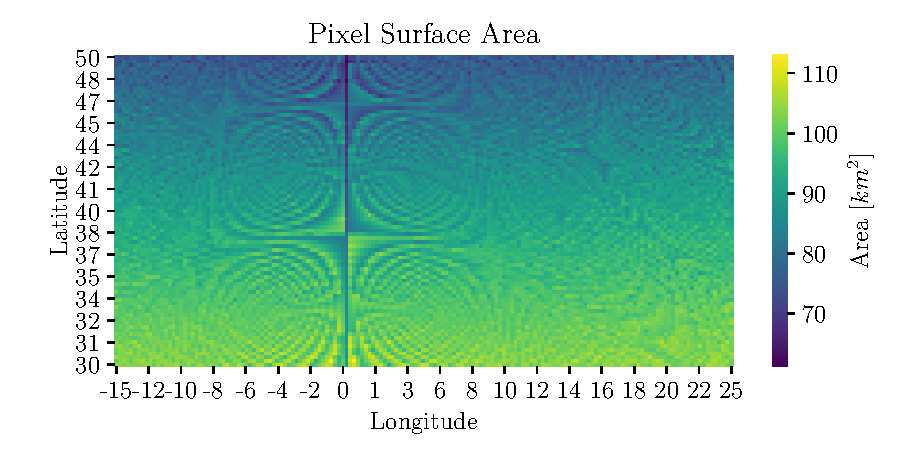
\includegraphics{python_figs/signal_area_pixel.pdf}
    \caption{The surface areas of pixels decreasing poleward. Note, the pattern appears to be more pronounced close to the meridian decreasing in both east and west direction.}
    \label{fig:area_pixel_signal}
\end{figure} 

\tdplotsetmaincoords{60}{110}
%
\pgfmathsetmacro{\rvec}{1.6}
\pgfmathsetmacro{\thetavec}{30}
\pgfmathsetmacro{\phivec}{60}

\pgfmathsetmacro{\deltathetavec}{40}
\pgfmathsetmacro{\deltaphivec}{80}

\begin{figure}
    \centering
    
    
\tdplotsetmaincoords{60}{110}
%
\pgfmathsetmacro{\rvec}{1.0}

\pgfmathsetmacro{\thetavec}{30}
\pgfmathsetmacro{\deltathetavec}{40}
\pgfmathsetmacro{\deltatwothetavec}{50}
\pgfmathsetmacro{\deltathreethetavec}{60}

\pgfmathsetmacro{\phivec}{-30}
\pgfmathsetmacro{\deltaphivec}{10}
\pgfmathsetmacro{\deltatwophivec}{50}
\pgfmathsetmacro{\deltathreephivec}{90}

\begin{tikzpicture}[scale=5,tdplot_main_coords]

    %%%%%%%%%%%%%% Setting up axis and coordinate system.
    \coordinate (O) at (0,0,0); % origo
    \coordinate (z) at (0, 0, \rvec); % origo
    %\draw[thin, <->] (1, 0.7, 1.16) -- (1, 0.52, 1.2) node[pos = 0.8, above right]{\Large $d\theta$};
    \draw[very thick,->, opacity = 1.] (0,0,0) -- (1.7, 0, 0) node[anchor=north east]{\Large $x$};
    \draw[very thick,->,  opacity = 1.] (0,0,0) -- (0, 1.7, 0) node[anchor=north west]{\Large $y$};
    \draw[very thick,->,  opacity = 1.] (0,0,0) -- (0, 0, 1.7) node[anchor=south]{\Large $z$};
    \shade[ball color = teal, opacity = 0.1] (0,0,0) circle [radius=\rvec];
    \draw (0,0,0) circle [radius=\rvec];

    %%%%%%%%%%%%%%%%%%%%%%%%%%%% first column
    \tdplotsetcoord{P}{\rvec}{\thetavec}{\phivec}
    \tdplotsetcoord{dP}{\rvec}{\deltathetavec}{\phivec}
    \tdplotsetcoord{G}{\rvec}{\thetavec}{\deltaphivec}
    \tdplotsetcoord{dG}{\rvec}{\deltathetavec}{\deltaphivec}
    
    \draw[dashed, very thick, color=teal, fill = teal, opacity = 0.2] (P) -- (dP) -- (dG) -- (G) -- (P);
    \draw[dashed, very thick, color=teal] (P) -- (dP) -- (dG) -- (G) -- (P);
    
    \tdplotsetcoord{a}{\rvec}{\deltathetavec}{\phivec}
    \tdplotsetcoord{b}{\rvec}{\deltatwothetavec}{\phivec}
    \tdplotsetcoord{c}{\rvec}{\deltathetavec}{\deltaphivec}
    \tdplotsetcoord{d}{\rvec}{\deltatwothetavec}{\deltaphivec}
    
    \draw[dashed, very thick, color=teal, fill = teal, opacity = 0.2] (a) -- (b) -- (d)-- (c) -- (a);
    \draw[dashed, very thick, color=teal] (a) -- (b) -- (d)-- (c) -- (a);
    
    \tdplotsetcoord{e}{\rvec}{\deltatwothetavec}{\phivec}
    \tdplotsetcoord{f}{\rvec}{\deltathreethetavec}{\phivec}
    \tdplotsetcoord{g}{\rvec}{\deltatwothetavec}{\deltaphivec}
    \tdplotsetcoord{h}{\rvec}{\deltathreethetavec}{\deltaphivec}
    
    \draw[dashed, very thick, color=teal, fill = teal, opacity = 0.2] (e) -- (f) -- (h)-- (g) -- (e);
    \draw[dashed, very thick, color=teal] (e) -- (f) -- (h)-- (g) -- (e);

    %%%%%%%%%%%%%%%%%%%%%%%%%%%%%%%% second column
      
    \tdplotsetcoord{P}{\rvec}{\thetavec}{\deltaphivec}
    \tdplotsetcoord{dP}{\rvec}{\deltathetavec}{\deltaphivec}
    \tdplotsetcoord{G}{\rvec}{\thetavec}{\deltatwophivec}
    \tdplotsetcoord{dG}{\rvec}{\deltathetavec}{\deltatwophivec}
    
    \draw[dashed, very thick, color=teal, fill = teal, opacity = 0.2] (P) -- (dP) -- (dG) -- (G) -- (P);
    \draw[dashed, very thick, color=teal] (P) -- (dP) -- (dG) -- (G) -- (P);
  
      
    \tdplotsetcoord{a}{\rvec}{\deltathetavec}{\deltaphivec}
    \tdplotsetcoord{b}{\rvec}{\deltatwothetavec}{\deltaphivec}
    \tdplotsetcoord{c}{\rvec}{\deltathetavec}{\deltatwophivec}
    \tdplotsetcoord{d}{\rvec}{\deltatwothetavec}{\deltatwophivec}
    
    \draw[dashed, very thick, color=teal, fill = teal, opacity = 0.2] (a) -- (b) -- (d)-- (c) -- (a);
    \draw[dashed, very thick, color=teal] (a) -- (b) -- (d)-- (c) -- (a);
  
  
    \tdplotsetcoord{e}{\rvec}{\deltatwothetavec}{\deltaphivec}
    \tdplotsetcoord{f}{\rvec}{\deltathreethetavec}{\deltaphivec}
    \tdplotsetcoord{g}{\rvec}{\deltatwothetavec}{\deltatwophivec}
    \tdplotsetcoord{h}{\rvec}{\deltathreethetavec}{\deltatwophivec}
    
    \draw[dashed, very thick, color=teal, fill = teal, opacity = 0.2] (e) -- (f) -- (h)-- (g) -- (e);
    \draw[dashed, very thick, color=teal] (e) -- (f) -- (h)-- (g) -- (e);
    
    
    %%%%%%%%%%%%%%%%%%%%%%%%%%%%%%%% third column
    \tdplotsetcoord{P}{\rvec}{\thetavec}{\deltatwophivec}
    \tdplotsetcoord{dP}{\rvec}{\deltathetavec}{\deltatwophivec}
    \tdplotsetcoord{G}{\rvec}{\thetavec}{\deltathreephivec}
    \tdplotsetcoord{dG}{\rvec}{\deltathetavec}{\deltathreephivec}
    
    \draw[dashed, very thick, color=teal, fill = teal, opacity = 0.2] (P) -- (dP) -- (dG) -- (G) -- (P);
    \draw[dashed, very thick, color=teal] (P) -- (dP) -- (dG) -- (G) -- (P);
  
    \tdplotsetcoord{a}{\rvec}{\deltathetavec}{\deltatwophivec}
    \tdplotsetcoord{b}{\rvec}{\deltatwothetavec}{\deltatwophivec}
    \tdplotsetcoord{c}{\rvec}{\deltathetavec}{\deltathreephivec}
    \tdplotsetcoord{d}{\rvec}{\deltatwothetavec}{\deltathreephivec}
    
    \draw[dashed, very thick, color=teal, fill = teal, opacity = 0.2] (a) -- (b) -- (d)-- (c) -- (a);
    \draw[dashed, very thick, color=teal] (a) -- (b) -- (d)-- (c) -- (a);
  
    \tdplotsetcoord{e}{\rvec}{\deltatwothetavec}{\deltatwophivec}
    \tdplotsetcoord{f}{\rvec}{\deltathreethetavec}{\deltatwophivec}
    \tdplotsetcoord{g}{\rvec}{\deltatwothetavec}{\deltathreephivec}
    \tdplotsetcoord{h}{\rvec}{\deltathreethetavec}{\deltathreephivec}
    
    \draw[dashed, very thick, color=teal, fill = teal, opacity = 0.2] (e) -- (f) -- (h)-- (g) -- (e);
    \draw[dashed, very thick, color=teal] (e) -- (f) -- (h)-- (g) -- (e);
    
    %%%%%%%%%%%%%%%%%%%%%%%%%% Adding coordinate information

    % First column
    \draw[thick](0.3, -0.25, 0.5)node[scale=0.8, rotate = -15]{$(i,j-1)$};
    \draw[thick](0.3, -0.17, 0.7)node[scale=0.8, rotate = -15]{$(i+1,j-1)$};
    \draw[thick](0.3, -0.3, 0.3)node[scale=0.8, rotate = -15]{$(i-1,j-1)$};

    % Second column
    \draw[thick](0.5, 0.3, 0.65)node[scale=0.8, rotate = 5]{$(i,j)$};
    \draw[thick](0.5, 0.3, 0.85)node[scale=0.8, rotate = 5]{$(i+1,j)$};
    \draw[thick](0.5, 0.3, 0.45)node[scale=0.8, rotate = 5]{$(i-1,j)$};
    
    % Third column
    \draw[thick](0.5, 0.73, 0.87)node[scale=0.8, rotate = 35]{$(i,j+1)$};
    \draw[thick](0.5, 0.8, 0.7)node[scale=0.8, rotate = 35]{$(i-1,j+1)$};

    \draw[thick](0.05, 0.45, 0.73)node[scale=0.8, rotate = 35]{$(i+1,j+1)$};

    \tdplotsetthetaplanecoords{\phivec};
    \shade[ball color=teal,tdplot_screen_coords,opacity=0.2] (O) circle[radius=\rvec];
    \foreach \X/\Y in {xy/z,yz/x,zx/y}
        {\begin{scope}[canvas is \X\space plane at \Y=\rvec]
         \fill circle[radius=1pt];
        \end{scope}}
    \end{tikzpicture}
    
    \caption{Sketch illustrating the relative size of neighboring pixels in uniform grid of \acrshort{ecc}, projected onto spherical coordinates. The areas of pixels in a uniform grid decrease poleward.}
    \label{fig:relative_size_neigbouring_pixels}
\end{figure}

\subsection{Verification of AWRS}
The regridding scheme is a set of algorithms. Before the production of the full dataset it is important to verify the correctness of the algorithms of \acrshort{awrs}.

%%%%%%%%%%%%%%%%%%%%%% TEST 1 - Formula to compute the area 
The computations of the areas are the foundation of the \acrshort{awrs}, and it is crucial to verify that the algorithm is correct. CDO (\cite{cdo}) provides functionality to compute grid areas of a uniform grid using the code inserted below.
\begin{verbatim}
$ cdo gridarea era5data.nc gridarea.nc     
\end{verbatim}
To verify the implementations of Equation \eqref{eq:sphere_finish}, the grid areas of \acrshort{era5} are computed using both CDO and the self implemented algorithm. Both versions produce the same results.
% må jeg skrive hvor like, TS: nei
Note that the self implemented code is scaled by $R$ to be consistent with CDO. Multiplication followed by division of the same number provides no additional information, and there is the off chance of introducing additional numerical errors. 

%%%%%%%%%%%%%%%%% TEST 2 -- vis regridding
A reason for confusion in the process of developing the \acrshort{awrs} algorithm arose from the different rotations of the data provided by the \acrshort{grib} and \acrshort{netcdf} files. The coordinate information is available in \acrshort{netcdf}, but the file-size is too large to store all data in this format, therefore the data is downloaded in \acrshort{grib}, as mentioned in Section \ref{sec:EUMETSAT_cloud_mask}. The \acrshort{grib}-file is provided as the left and right flipped version of the  \acrshort{netcdf}-file. A fast modular test to check the regridding routine is to insert the raw data including the land and sea masks. Figure \ref{fig:visual_inspection_regridding} shows a example of the regridding of the raw data from 2\textsuperscript{nd} May 2009. Clouds are illustrated in white, land mask in teal and sea in purple. The original data also include the category off-earth disk, this is not a member of the chosen subset. By regridding the raw data it quickly becomes apparent whether the correct domain has been used, and evident if the algorithm generates any discontinuities in space. 
\begin{figure}
    \centering
    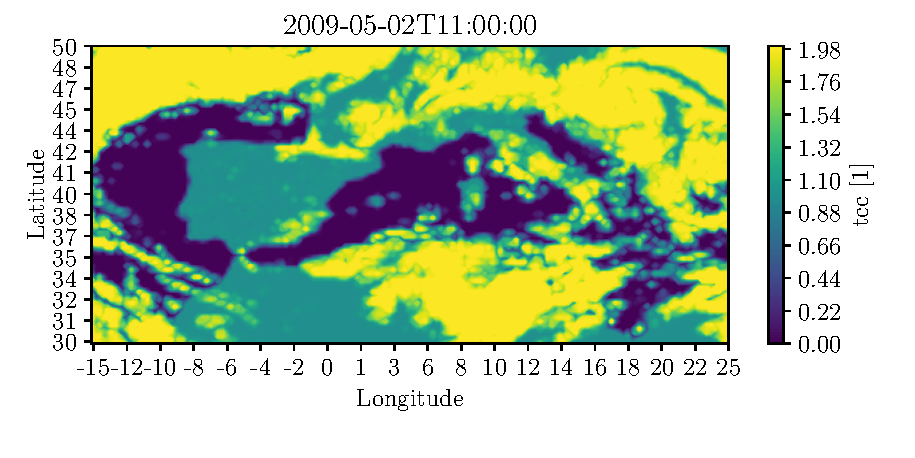
\includegraphics{python_figs/visual_regridding.pdf}
    \caption{Result from regridding the raw product, which includes land and sea masks in the absence of clouds. Land is illustrated in teal, sea in purple and clouds in white.}
    \label{fig:visual_inspection_regridding}
\end{figure}

\subsection{Missing Data} \label{sec:missing_values}
Missing values are inevitable when working with observational data. Sensors occasionally fail to collect measurements and data is missing. This can either be individual pixels or entire disks. In this project single NaN values are no pressing issue since they are remapped to fractions by using the area weighting of the other values. Contributing NaN pixels are counted and stored for future use in \acrshort{ecc}.
\begin{figure}
    \centering
    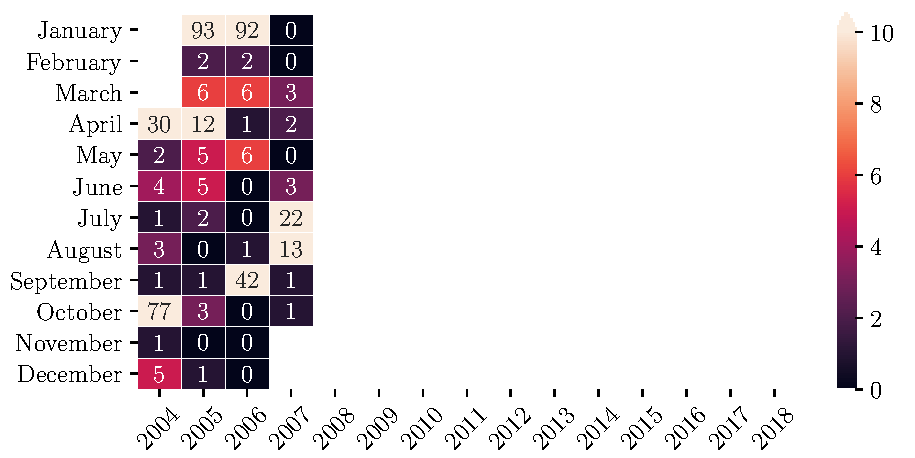
\includegraphics[scale = 1.0]{python_figs/heatmap_missing_values.pdf}
    \caption{Heatmap summarising missing hours per month for all years.}
    \label{fig:heatmap_missing_values}
\end{figure}
\begin{figure}
    \centering
    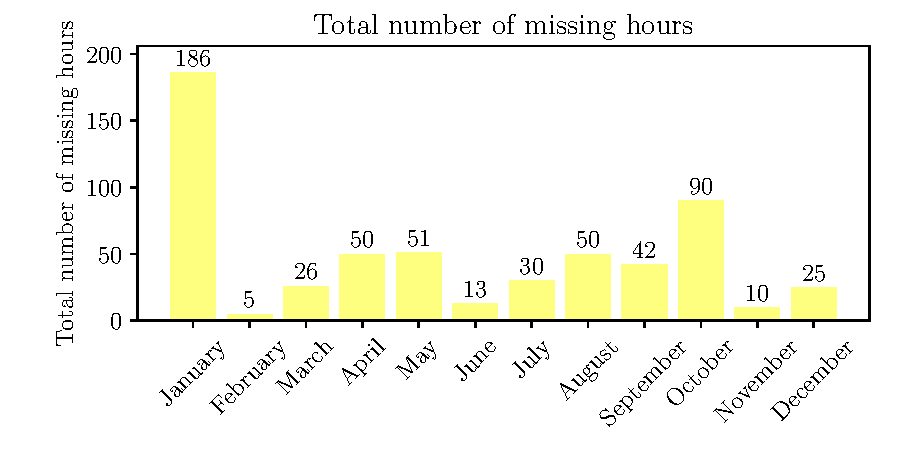
\includegraphics[scale = 1.0]{python_figs/heatmap_missing_values_monthly_sum.pdf}
    \caption{Barplot showing the monthly sum of missing values. This excludes the contribution from the period of 2004 before the satellite was operational.}
    \label{fig:barplot_missing_values}
\end{figure}
In some cases the sensor fails to scan and in other cases the data has been destroyed prior to archiving. Independent of the cause, the result is the same, the data can never be recovered. Further down the chain of supply, the missing data can cause issues for the process of downloading data. Corrupt data can enter infinity loops without being detected by \acrshort{eumetsat}. One request amount to approximately 3.5 months of hourly data. The combination of corrupt data and maximum number of pending requests (20) have cause some delays in preparing the dataset. 

Missing timestamps result in missing disks. When available the closest time step within the previous and trailing 45 minutes is used to fill the gap. A summary of missing values per month in the data set is provided in Figure \ref{fig:heatmap_missing_values}. Aggregation of missing values per month is presented in Figure \ref{fig:barplot_missing_values}. The plot is ment to illustrate any seasonal biases. The months of 2004 prior to the time at which the satellite became operational are not included in the statistics of missing values.

METeosat provides a two satellite system, and occasionally both the standby and the operational sensors scan at the same time, as mentioned in Section \ref{sec:meteosat}.
In cases of technical failures, the standby scan is used. The scans are done from a different nominal position. However, the coordinate systems remain the same, since the standby scan is rectified to the position of the operational satellite before the product is released (personal communication \acrshort{eumetsat} staff). Comparing simultaneous measurements for the operational and the standby METeosat satellites, it becomes clear that they are dissimilar. However, this does not occur very frequently and there has been no effort in quantifying the magnitude of the parallax, to correct for the bias this may introduce.

Manually generated datasets are prone to human error, especially in the case where users need to download individual time steps to fill the gaps. The instances of missing values were double checked. In summary the workflow has been as follows: the author downloaded the data, detected missing times and manually chose the closest time step available within the previous and trailing 45 minutes. In retrospect, the downloading options (API or GUI) provided by the satellite service should be taken into account when choosing the data.

\subsection{Masks} \label{sec:mask}
The land sea masks are provided by \acrfull{metno}. In its original format the masks have a $0.1^o$ resolution and global coverage, not including the polar regions. These are regridded to a suitable resolution of $0.25^o$ using functionality available in PyAEROCOM (\cite{pyaerocom}). %(\href{https://pyaerocom.met.no/}{https://pyaerocom.met.no/}). 
This is a python toolbox developed within the \acrfull{aerocom} project. To avoid storing redundant data, only domain specific data is made available in the project supplementary repository. For more details on supplementary material, see Section \ref{sec:structure_and_implementations}.
%To keep memory-requirements to a minimum only the parts of the filters relevant domain is stored in the supplementary material for this project.
\begin{figure}
    \centering
    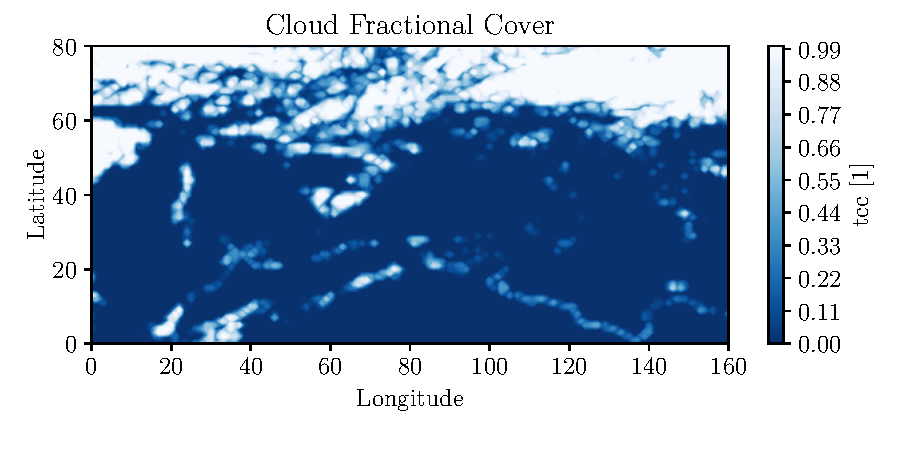
\includegraphics{python_figs/example_artefact.pdf}
    \caption[Artifact in European Cloud Cover dataset.]{The results after regridding reveal an artifact. This is a snapshot from May 2\textsuperscript{nd} 2004 at noon. The frequency of occurrence is currently unknown.}
    \label{fig:example_artifact}
\end{figure}

Filters available in the supplementary material are \textit{land}, \textit{sea}, \textit{coastline} and \textit{artifact}. The coastline is defined to be all pixels that are not either 100\% land or sea. A threshold based binary classification is used to separate the coastline pixels into land or sea. The threshold is set to 50\%. Pixels containing at least 50\% of sea are most likely affected by maritime conditions, making it reasonable to classify them as sea pixels.
\begin{figure}
    \centering
    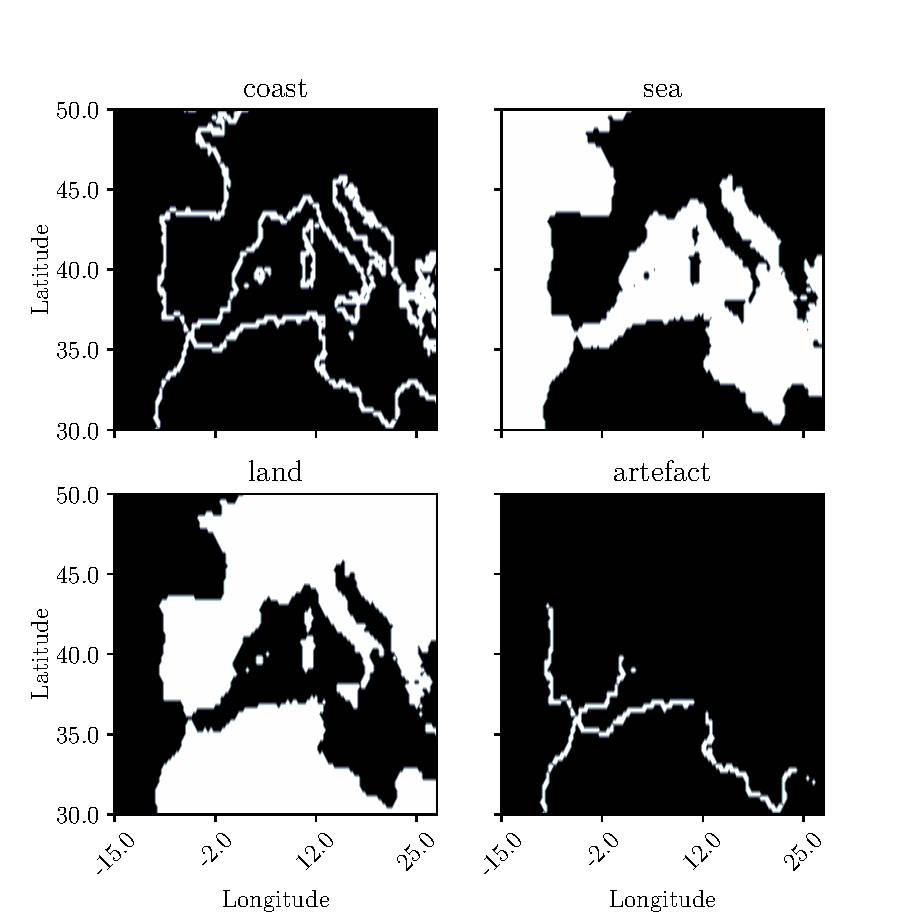
\includegraphics{python_figs/filters.pdf}
    \caption{Figure shows all filters, in white, available in the python package ``sciclouds''.}
    \label{fig:filters_subplot}
\end{figure}

Based on a visual comparison to Figure \ref{fig:example_artifact}, the artifact is defined to be all coastline pixels obeying the following inequality.
\begin{equation} \label{eq:artifact_condition}
    \theta + \frac{1}{3}\phi < 40
\end{equation}
All filters are displayed in Figure \ref{fig:filters_subplot}. 
%shows a subplot of all filters, including the artifact detecting filter. 
The signal from the artifact filter when applied to \acrshort{ecc} seem to follow a normal distribution as shown Figure \ref{fig:signal_artifact} in Appendix \ref{app:misc}. To get an idea of the frequency of appearance, it is necessary to detect when it appears in isolation and not in cloud. It could, for instance, be done by studying the histograms from the ratio of the artifact signal and a buffered artifact filter. No efforts have been made to remove the artifact from the data. 

\subsection{Statistical Properties in ECC}
To summarize and present the content of \acrshort{ecc}, statistical properties are used. For clarity, the period used in this section is 2004 to 2018. The properties selected in this study are mean, minimum (min), maximum (max), median, \acrfull{std} and \acrfull{mad}. The most important results are presented in this section, and complementary figures can be found in the Appendix \ref{ch:appendix_statistic}. 
The data varies in space an time. Statistical properties are calculated over one or both of these axes.

\subsubsection{Statistics over space and time} 
%%% BAR PLOT GLOBAL STATISTICS
To study the statistical properties at different parts of the domain the filters, shown in Figure \ref{fig:filters_subplot}, were applied to the data before computing the statistical properties. Figure \ref{fig:bar_plot_global_stats} shows a barplot summarizing the statistical properties for the five variables (Temperature, Surface Pressure, Cloud fractional cover, Specific and Relative humidity) and four filters (coast, land, sea and all). It shows minor differences between the statistical properties applied. The largest difference can be seen in the maximum value of relative humidity, where the maximum above land is larger than that above sea. The relative difference in magnitude between \acrshort{mad} and \acrshort{std} and the other variables from the reanalysis dataset, is solid. Most likely because the data is smoothed as a consequence of using assimilation model. 
\begin{figure}[ht]
    \centering
    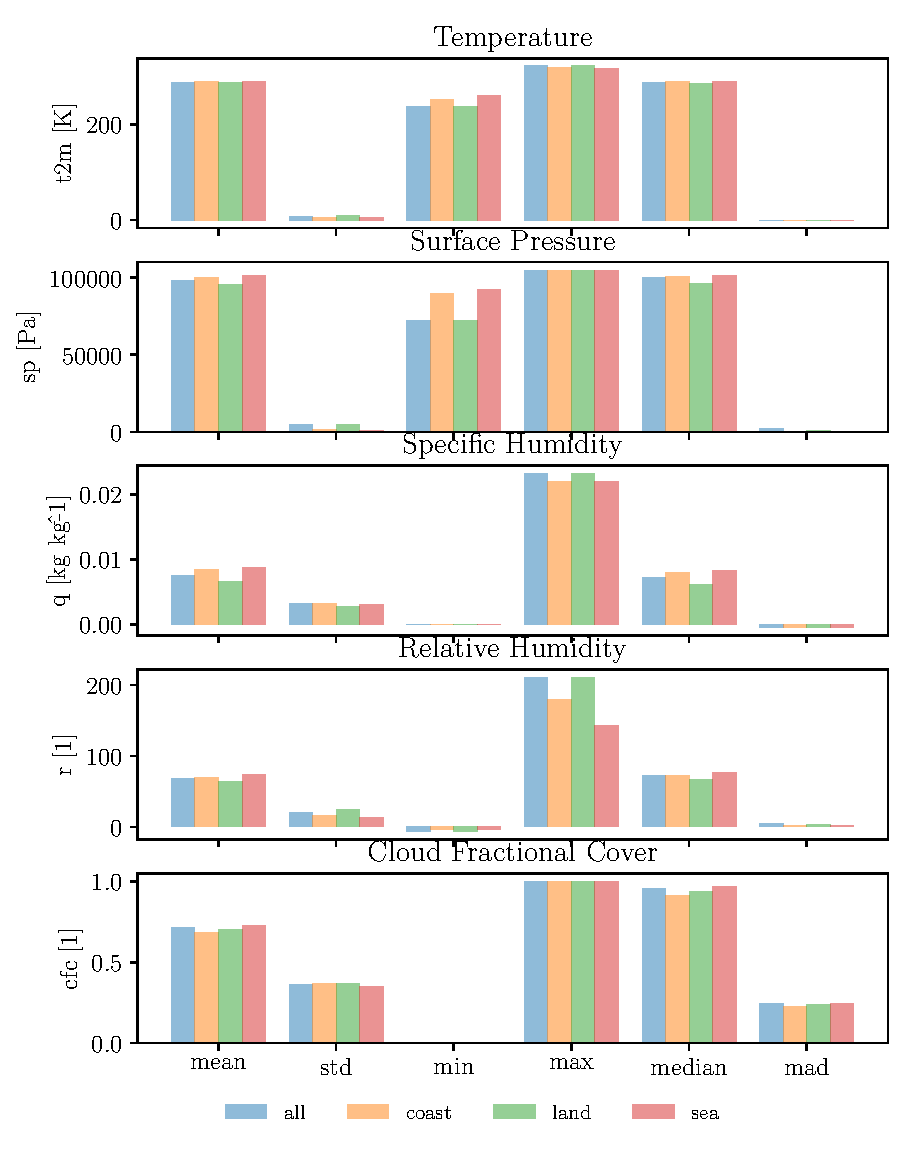
\includegraphics{python_figs/bar_plot_global_statistics_new_legend.pdf}
    \caption{Bar plot showing global statistics for different filters.}
    \label{fig:bar_plot_global_stats}
\end{figure}

\subsubsection{Temporal statistics}
%%%%%%%%%%%%%%%%%%%%%%%%%%%%%%%%%%% MONTHLY MEANS
Figure \ref{fig:monthly_mean_ts_vars} shows the spatially averaged monthly mean values for all variables. Seasonal effects and differences between land and sea are evident among all variables. For temperature and relative humidity, a more pronounced seasonal cycle over land, compared to sea, is evident. The remaining variables appear to have a small shift towards higher values over the sea. This is as expected, the pressure decrease with altitude and the sea is a source of humidity. On a monthly average the temperature over land is higher than the sea, but the difference is small, a couple degrees.
%On a global scale the ocean is significantly more cloudy than land. Keep in mind that most clouds are consentrated in storm tracks, the North Atlatic Storm Track may grace this domain, but it is not on its main trajectory.
\begin{figure}[ht]
    \centering
    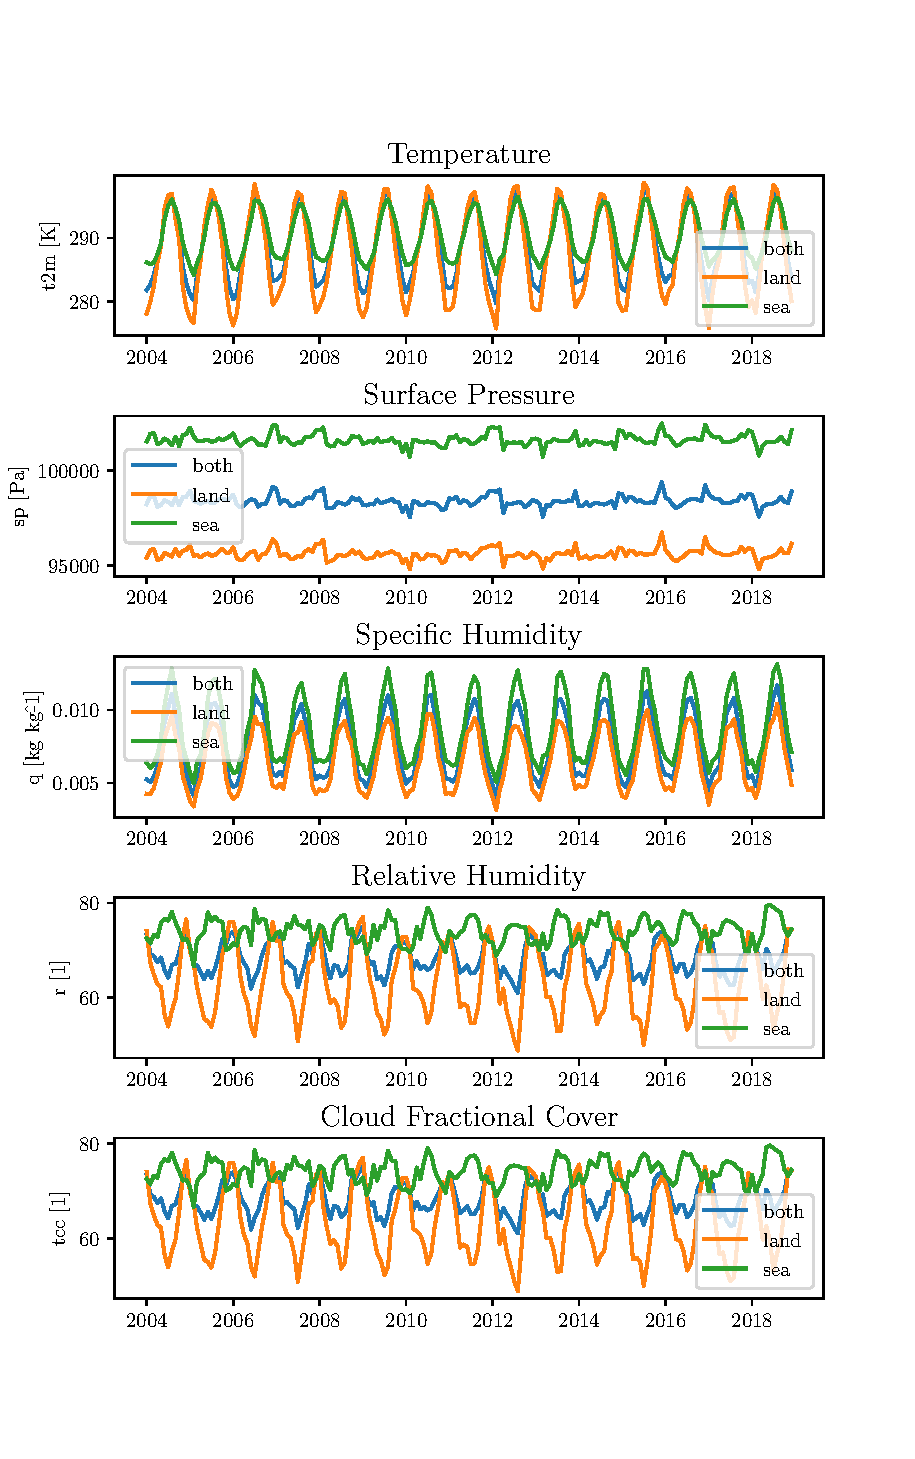
\includegraphics{python_figs/monthly_means.pdf}
    \caption{Spatially averaged monthly values. Filters are applied for land and sea.}
    \label{fig:monthly_mean_ts_vars}
\end{figure}

%As a reference the global cloud cover over land is X and over sea is Y. 
The spatially averaged time series for the first week of September in 2012 is shown in Figure \ref{fig:first_week_sep_2012}, illustrating the relative strength of the signal fed into the input sequence. As a reference, the signals over land and sea are provided. All variables display diurnal variations. 
\begin{figure}[ht]
    \centering
    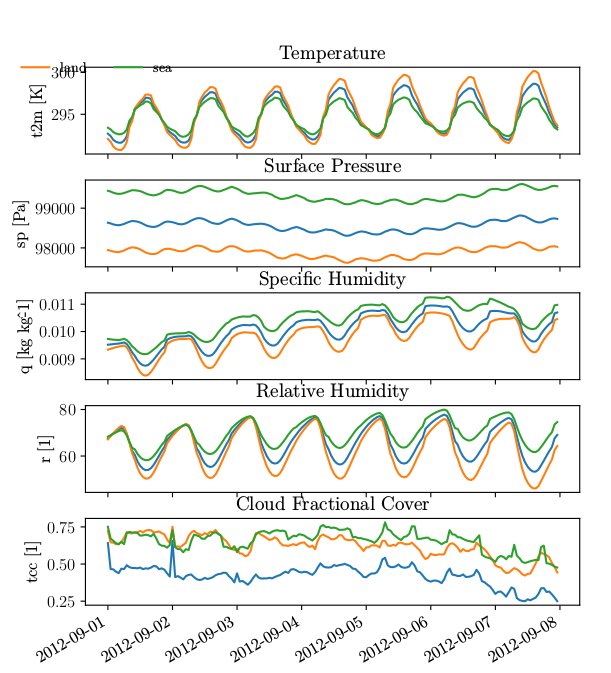
\includegraphics{python_figs/spatially_averaged_one_week_from_2012-09-01.png}
    \caption{Spatially averaged time series, showing the evolution of cloud cover and other variables in the first week of September 2012.}
    \label{fig:first_week_sep_2012}
\end{figure}
The figure shows small diurnal variations over sea, for all variables except clouds. In this week in September 2012, the temperature in \acrshort{era5} is remarkably constant. Varying within one degree and the temperature at sea, nothing at all. Recall, this is hourly reanalysis data. The variables, excluding clouds, show little variation, the amplitudes are nearly constant and the lines of values don't cross each other. 
%The case for most, mean follow the data over land, with a smaller amplitude. The mean gets smoothed by the small diurnal variations over land. 

The complete series of first weeks of the remaining months of 2012 is shown in Appendix \ref{app:first_week}. Under the assumption that the first week of a month is representative for that month. This series show that the diurnal changes of temperature and relative humidity vary most within the course of the year. 

\begin{figure}
    \centering
    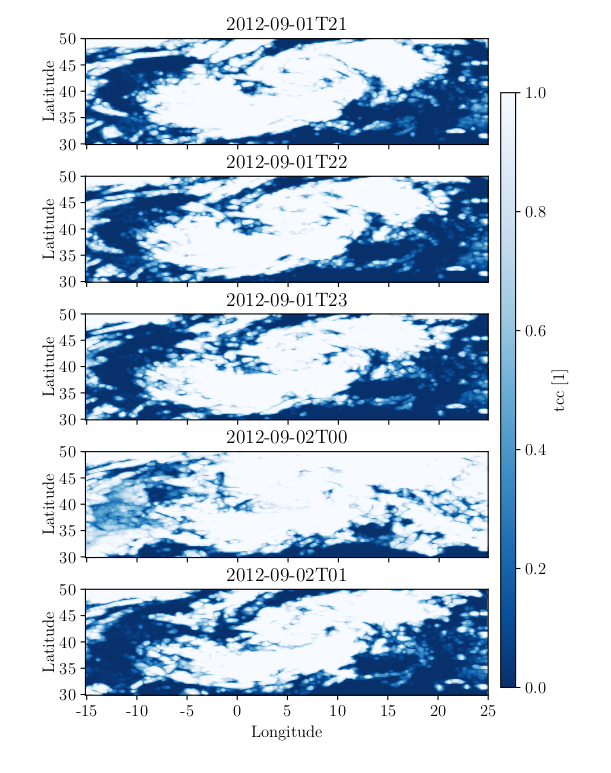
\includegraphics{python_figs/timelapse_tcc_spike_09_2012.png}
    \caption{Evolution of the spike detected in Figure \ref{fig:first_week_sep_2012}.}
    \label{fig:spike_sep_2012}
\end{figure}
Note the spike appearing on September 2\textsuperscript{nd} in Figure \ref{fig:first_week_sep_2012}. To examine this event Figure \ref{fig:spike_sep_2012} was produced. From studying the evolution of the cloud cover it doesn't appear to be a numerical artifact. It is simply looks like there is a low pressure system centered in Europe, able to raise the cloud cover from 0.4 to 0.7 within one hour. Recall from Section \ref{sec:ecc} that low pressure system swirls counter clockwise north of Equator. 

\subsubsection{Temporal statistics}
All the statistical properties computed over time for the variable \acrshort{cfc} in \acrshort{ecc} are plotted in 
Figures \ref{fig:all_stats_tcc} and \ref{fig:deviation_tcc}. Similar figures for the remaining variables in the dataset are presented in Section \ref{sec:all_stats}. 
With the exception of minimum and maximum values, the cloud cover is affected by the coastline, on average there is a lower cloud fractional cover at the coast. In large regions the median value is one, revealing that in these areas more than half of the datapoints are 1.
% This is surprising? 
%% CLOUD FRACTIONAL COVER
\begin{figure}[ht]
    \centering
    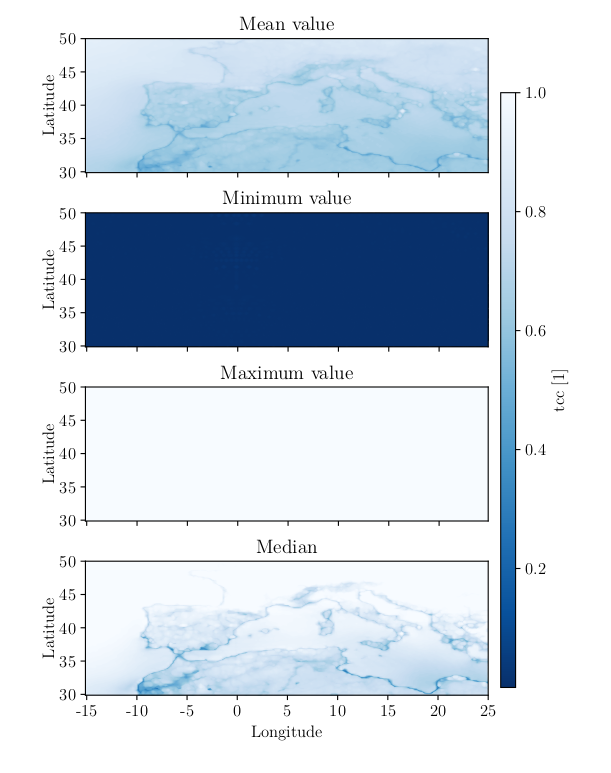
\includegraphics{python_figs/all_stat_variable_tcc.png}
    \caption{Contour plot showing the local (pixel) statistics for cloud fractional cover.}
    \label{fig:all_stats_tcc}
\end{figure}
\begin{figure}
    \centering
    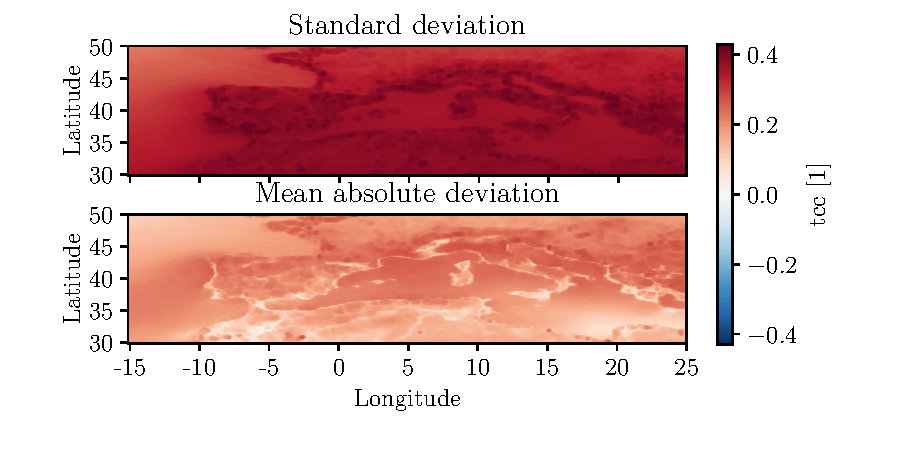
\includegraphics{python_figs/DEVIATION_all_stat_variable_tcc.pdf}
    \caption{Deviations in  cloud fractional cover.}
    \label{fig:deviation_tcc}
\end{figure}

The mean values displayed in figure \ref{fig:all_stats_tcc} show that on average the coastline has a lower cloud cover than the adjacent areas. This is supported by the bar plot, see Figure \ref{fig:bar_plot_global_stats}. 
%From the minimum values of \acrshort{cfc} it becomes evident that there is another artifact present in the dataset. This pattern is most likely caused by the remapping routine. However by looking at the axis it is incrementally small and is not likely to affect the quality of the dataset much.

Figure \ref{fig:area_pixel_signal} shows the patterns of magnitude of the areas contributing to a pixel. One might expect all pixels to be without cloud cover for at least one hour over the period of 14 years, but this is not the case. The maximum value is as expected, one over the entire region, indicating that at some point every pixel is full of clouds. The standard deviation is higher over land, this is caused by larger variation in cloud cover in these regions. The median and \acrshort{mad} 
% Det er jo ikke rart for mad er medianen av en differanse.
show similar patterns, this is not surprising since \acrshort{mad} is short for \acrlong{mad}, where the lowest values are found along the coast.

\subsubsection{Correlation between cloud cover and environmental variables}
%%% CORRELATION
Correlation describes how strongly a pair of variables are linearly related. A positive correlation tells you that an increase in one variable results in an increase in the other. A negative correlation describes the opposite connection, implying that an increase in one variable causes a decrease in the other.
\begin{figure}[ht]
    \centering
    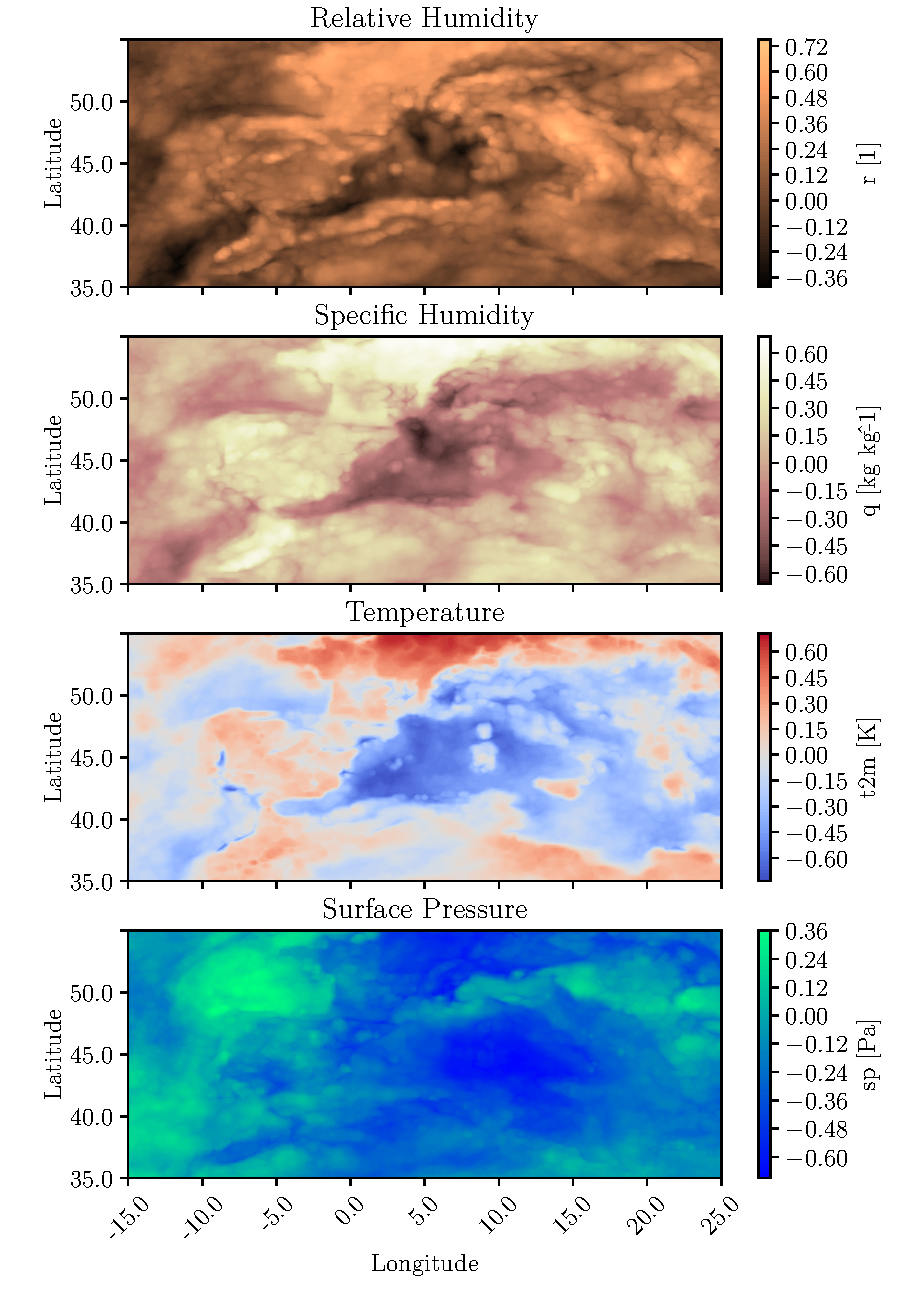
\includegraphics{python_figs/correlation_figure.pdf}
    \caption{Contour plot showing the correlation coefficient between environmental variables and cloud fractional cover.}
    \label{fig:correlation_tcc_vs_envio}
\end{figure}

The linear correlation coefficients from pairs of cloud cover and environmental variables such as temperature, pressure, relative and specific humidity are shown in Figure \ref{fig:correlation_tcc_vs_envio}. Recall that all environmental variables are produced by a reanalysis. Pink illustrates negative correlation while green illustrates a positive correlation. Note that different patterns emerge from all variables. %, implying that they could be useful as predictors. 

Over land relative humidity is dominated by positive correlation with cloud cover, although some parts of Africa and the sea in the eastern Mediterranean have a negative correlation. The image of the surface pressure is remarkably similar, showing a similar pattern but with opposite signs. The negative sign seems reasonable, since high pressure is often associated with sinking motions in the atmosphere and clouds are formed by rising motions. 

Specific humidity shows a clear shift at longitudinal degree 10. The land area in the west shows positive correlation with cloud cover while the eastern part shows a negative correlation. 

In most locations temperature is negatively correlated with cloud cover except in parts of the Alps, north coast of France and in north Africa. This seems reasonable since warmer air can retain more vapor.%, on the other hand this could enhance evaporation rate, making more vapor available for condensing onto particles. 


% Finished regriddidng files.
\subsection{Summary}
\acrshort{ecc} is comprised of five variables; temperature, pressure, cloud fractional cover, relative and specific humidity. These are collected from two sources; \acrshort{era5} and \acrshort{eumetsat}. The resolution available in \acrshort{era5} was preserved, while remapping the cloud mask to cloud fractional cover. 
% duplication
The final product consist of %the variables temperature, pressure, cloud fraction, specific humidity and relative humidity, available
hourly data on a $0.25^o$ uniform grid resolution in the period from April 2004 to December 2018. Cloud fractional cover (\acrshort{cfc}) is produced from area weighting cloud masks. The \acrshort{awrs} is described in Section \ref{sec:remapping}. The remaining variables are on their original format as provided by \acrfull{ecmwf}. A summary of the original sources of the dataset is given in Table \ref{tab:dataset_summary}. More details on \acrshort{era5} is available in Section \ref{sec:era5} and for the cloud mask in Section \ref{sec:EUMETSAT_cloud_mask}. 
\clearpage
\begin{table}[]
    \centering
    \resizebox{\textwidth}{!}{%
\begin{tabular}{c|c|c|c|c|}
\cline{2-5}
\multirow{4}{*}{}                                 & \multicolumn{2}{c|}{\textbf{ERA5}}                                                                                                   & \multicolumn{2}{c|}{\textbf{MSG2}}                                                                                                                \\ \cline{2-5} 
                                                  & \textbf{Type}                     & \textbf{Variables}                                                                               & \textbf{Type}                                                               & \textbf{Variables}                                                  \\ \cline{2-5} 
                                                  & Surface                           & \begin{tabular}[c]{@{}c@{}}2m Temperature\\ Surface pressure\end{tabular}                        & \multirow{2}{*}{Satelite retrival}                                          & \multirow{2}{*}{Cloud Mask}                                         \\ \cline{2-3}
                                                  & 1000 hPa                          & \begin{tabular}[c]{@{}c@{}}Relative Humidity\\ Specific Humidity\end{tabular}                    &                                                                             &                                                                     \\ \hline
\multicolumn{1}{|c|}{\textbf{Projection}}         & \multicolumn{2}{c|}{Uniform grid}                                                                                                    & \multicolumn{2}{c|}{Curve linear grid}                                                                                                            \\ \hline
\multicolumn{1}{|l|}{\textbf{Spatial resolution}} & \multicolumn{2}{c|}{$0.25^o$}                                                                                                        & \multicolumn{2}{c|}{-}                                                                                                                            \\ \hline
\multicolumn{1}{|c|}{\textbf{Output Frequencey}}  & \multicolumn{2}{c|}{Hourly}                                                                                                          & \multicolumn{2}{c|}{15 min}                                                                                                                       \\ \hline
\multicolumn{1}{|c|}{\textbf{Availability}}       & \multicolumn{2}{c|}{\begin{tabular}[c]{@{}c@{}}1979-onwards\\ Expected to be available from \\ 1950 some time in 2020.\end{tabular}} & \multicolumn{2}{c|}{2004-onward}                                                                                                                 \\ \hline
\multicolumn{1}{|c|}{\textbf{License}}           & \multicolumn{2}{c|}{\begin{tabular}[c]{@{}c@{}}Open Access. Need user \\ from Copernicus Data Storage.\end{tabular}}                  & \multicolumn{2}{c|}{\begin{tabular}[c]{@{}c@{}}Researcher Licences\\ to get 15min resolution.\\ Open access at \\ hourly resolution\end{tabular}} \\ \hline
\end{tabular}
}
\caption{Data description on the data present in the dataset ECC (European Cloud Cover). \textbf{Add projection as a column, Availability for download and the period of data.} There is a lot of work in combining the two datasets and processing it.}
\label{tab:dataset_summary}

\end{table}